\chapter{Rappel sur l'oscillateur harmonique}

Considérons le cas de l'oscillateur harmonique amorti :
\begin{dmath}
    \ddot{x} + \gamma\dot{x} + \omega_0^2 x = 0
    \qquad {\gamma > 0}
\end{dmath}   

Lorsque $\omega_0 > \frac{\gamma}{2}$ le système oscille de manière pseudopériodique et admet des solutions de la forme :

\begin{dmath}
    x(t) = e^{-\frac{\gamma}{2}t}(A\cos(\omega_{\gamma} t) + B\sin(\omega_{\gamma} t))
    \qquad {\omega_{\gamma} = \sqrt{\omega_0^2 - \gamma^2/4}}
\end{dmath}

Cette solution est caractérisé par des oscillations sinusoïdales avec une amplitude qui décroît de manière exponentielle selon $e^{-\frac{\gamma}{2} t}$.

\section{L'oscillateur forcé}

Étudions le cas où l’on applique une force periodique de la forme $f_0\cos(\omega t)$ :

\begin{dmath}
    \ddot{x} + \gamma\dot{x} + \omega_0^2 x = f_0\cos(\omega t)
    \label{eq:forced_osc}
\end{dmath}



Étant donné que la fréquence $\omega$ de la force ne correspondant 
géneralement pas à la fréquence naturelle de l'oscillateur $\omega_0$, 
elle ne se mettra pas à osciller 
On s'attend a ce pour grand t, $x$ finisse par adopter la 
fréquence d'oscillations $\omega$. 
On cherche une solution particulière de cette forme en passant 
par les complexes \cite{feynman_feynman_nodate}.

\begin{equation}
    x(t) = \Re(z(t)) \quad z(t) = Ae^{i\omega t}
\end{equation}

L'équation \eqref{eq:forced_osc} devient :

\begin{equation}
    (-\omega^2 + i\omega\gamma + \omega_0^2)z = f_0 e^{i\omega t}
\end{equation}

\begin{equation}
    z(t) = R f_0 e^{i \omega t} \qquad R = \frac{1}{\omega_0^2 - \omega^2 + i\omega\gamma} = \rho e^{i\phi}
\end{equation}

Le module $\rho$ est le multiplicateur d’ampltitude en réponse à la force, et l’argument $\phi$ va induire un déphasage de $x$ par rapport à la force.

En revenant dans les réels :
\begin{equation}
    x(t) = \rho f_0 \cos(\omega t + \phi)
    \qquad \dot{x}(t) = -\omega \rho f_0 \sin(\omega t + \phi)
\end{equation}

On peut déteminer les expressions pour $\rho$ et $\phi$

\begin{dmath}
    \rho^2 = RR^* \\
    = \frac{1}{(\omega_0^2 - \omega^2) + \omega^2\gamma^2}
\end{dmath}

\begin{dmath}
    \tan(\frac{\phi}{2}) = \frac{-\rho\omega\gamma}{\rho(\omega_0^2 - \omega^2) + 1}
\end{dmath}

\begin{figure}[!t]
    
    \subcaptionbox{}[.5\linewidth]{%
      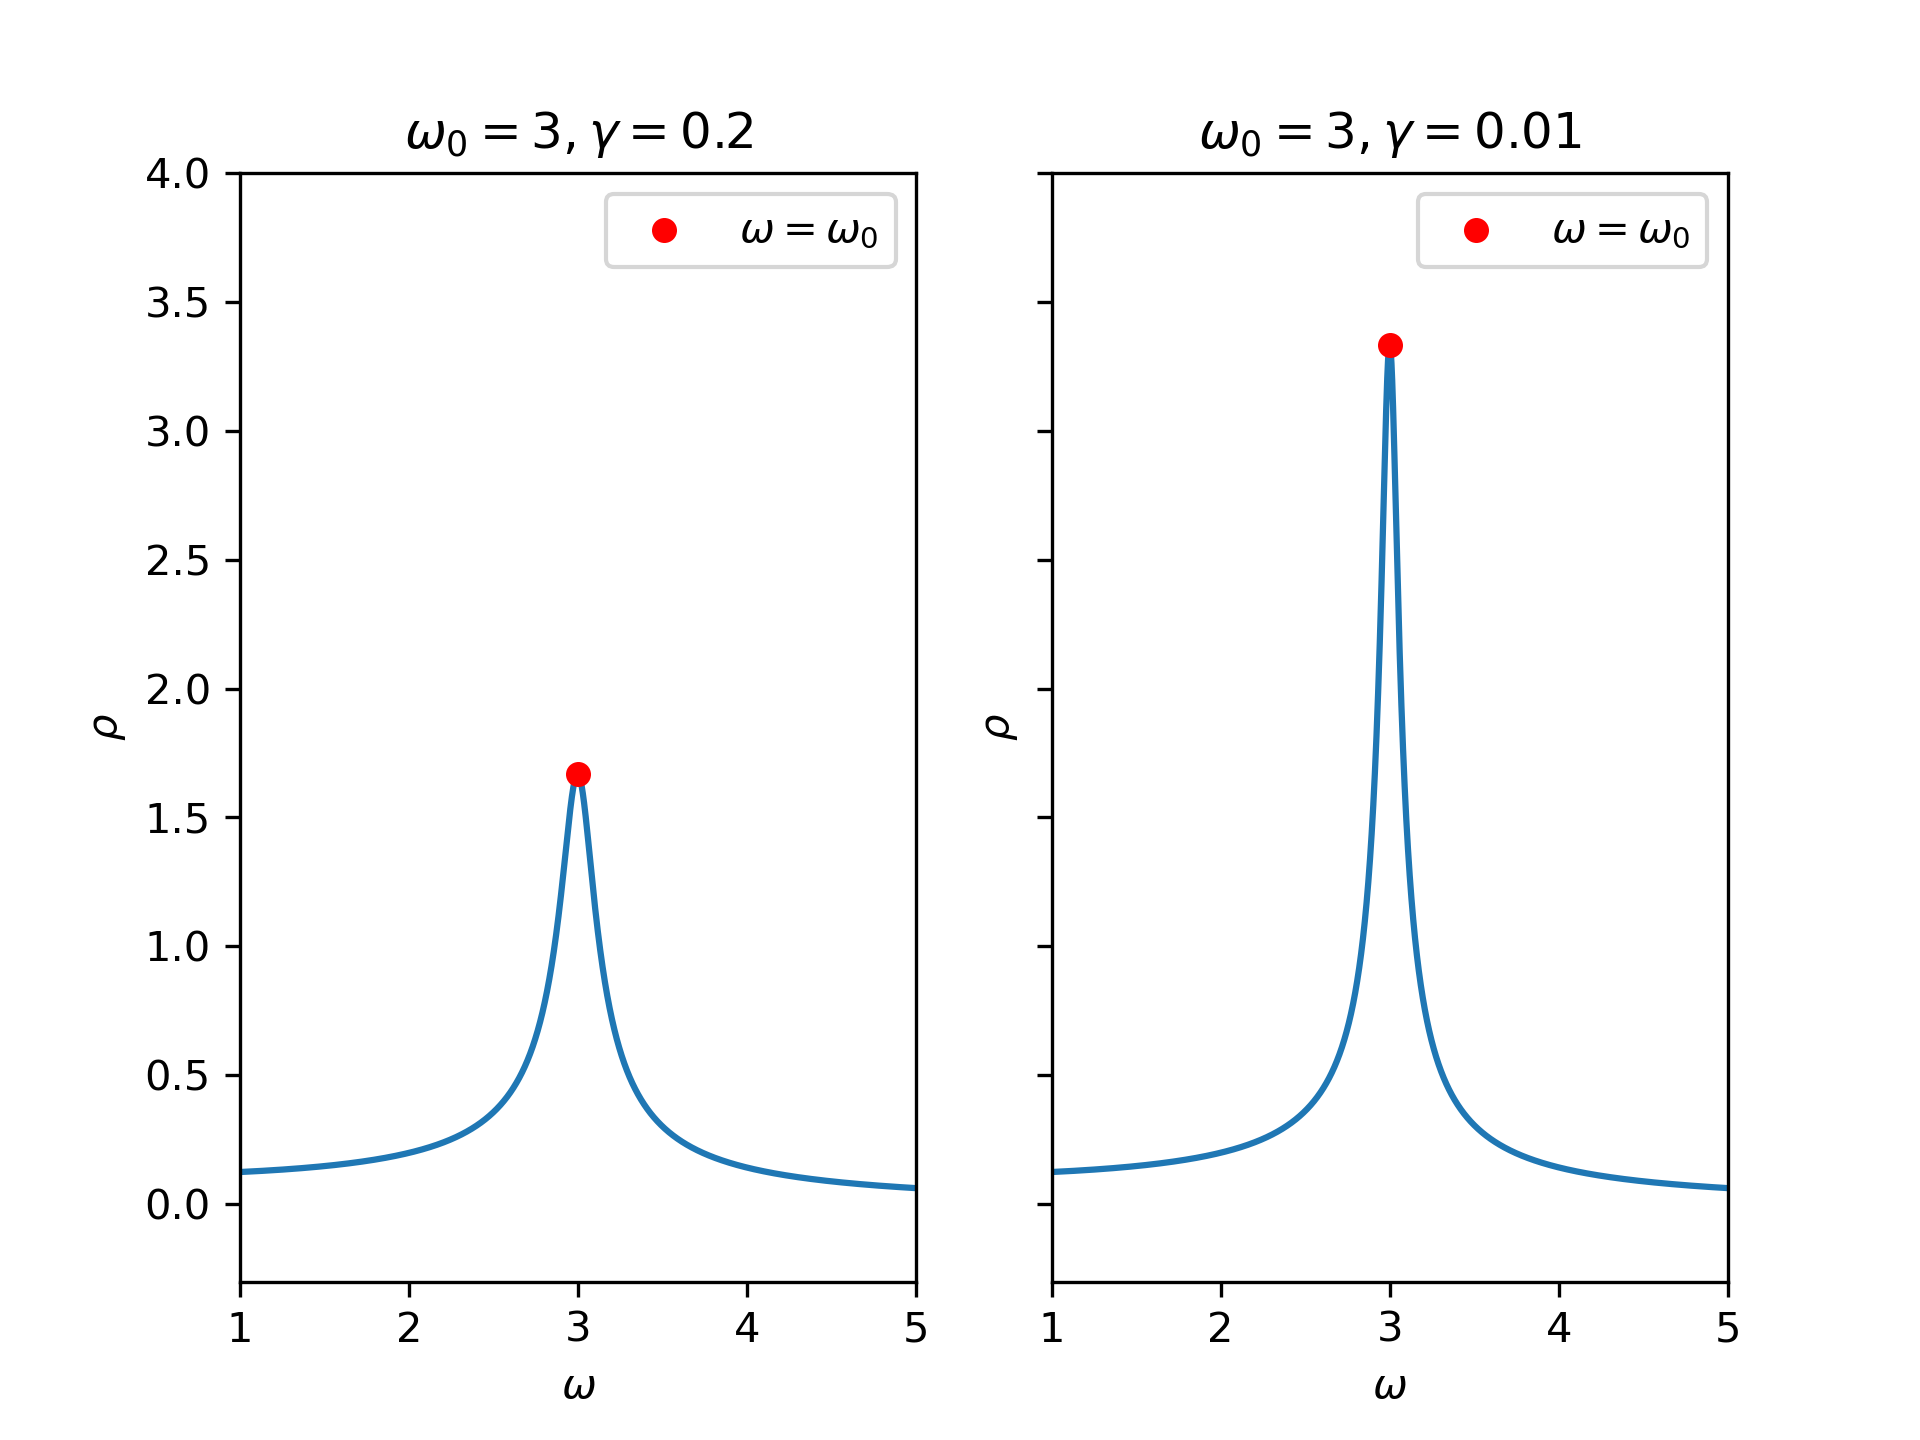
\includegraphics[width=\linewidth]{images/harmonique/rho_plot_contrast.png}%
      
    }%
    \hfill
    \subcaptionbox{}[.5\linewidth]{%
      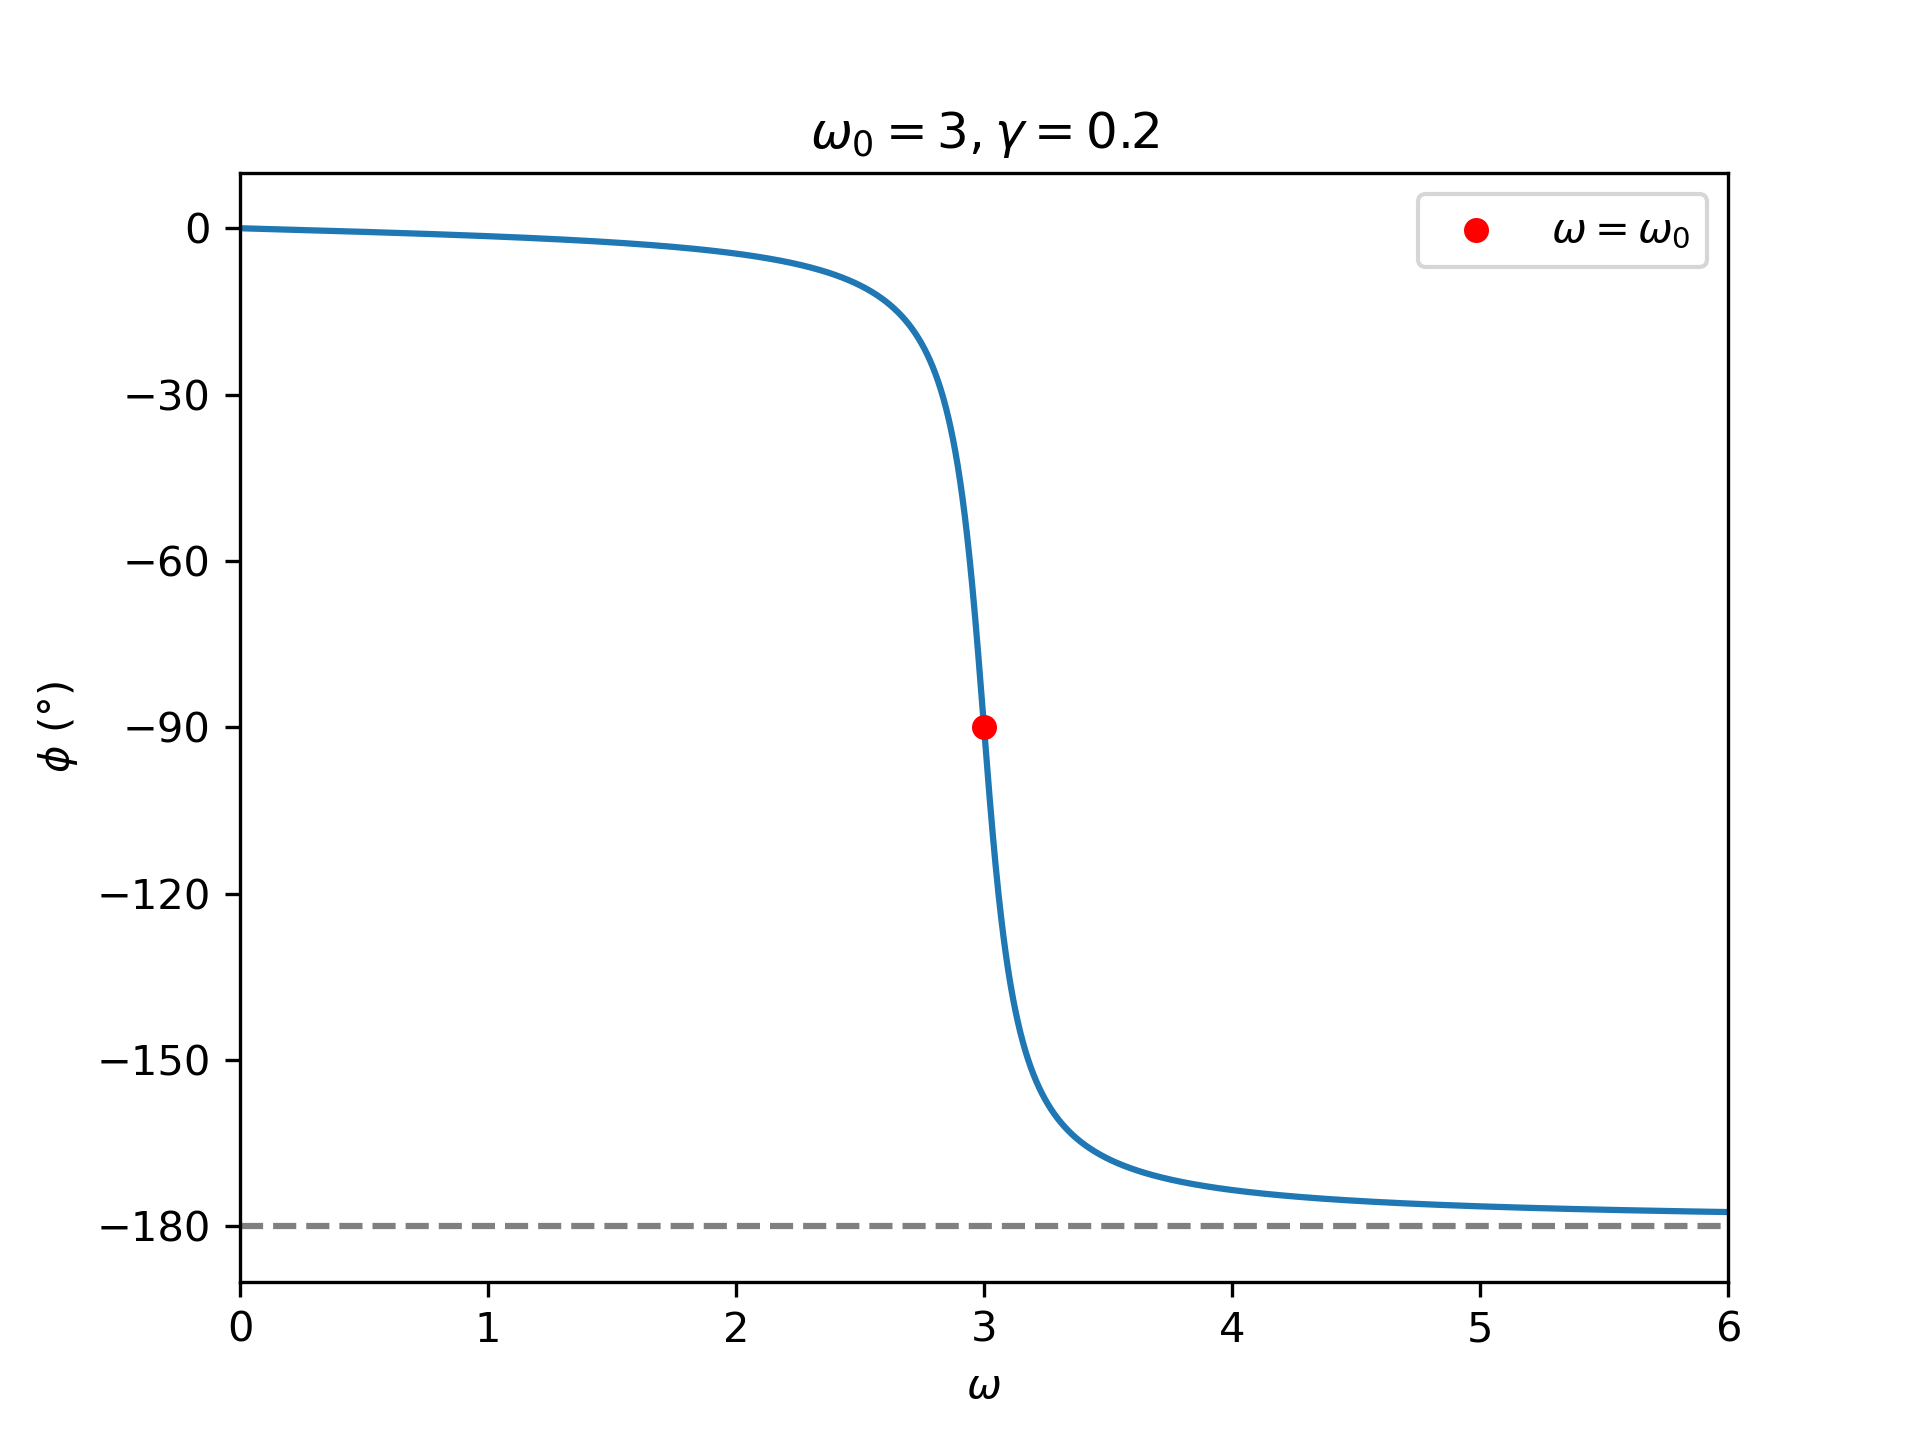
\includegraphics[width=\linewidth]{images/harmonique/frequency_phase_shift.png}%
      
    }
    \caption{\textbf{(a)} Résponse fréquentielle lorentzienne autour de la résonance. \textbf{(b)} Différence de phase en fonction de la fréquence.}
\end{figure}


%MONTRER PLOTS, PARLER DE LA LORENZTIENNE

$\rho$ prend la forme d’une courbe lorentzienne, l’amplification 
de la force est très forte lorsque $\omega$ est proche de $\omega_0$ 
(effet de résonance), l’amplification tend rapidement vers zero 
le plus $\omega$ s’éloigne de $\omega_0$.

Étant donné que la solution homogène tend vers $0$, à long terme l'oscillateur va atteindre un état stable où il sera synchronisé avec la force.